\section{夸克胶子等离子体}
\label{夸克胶子等离子体}
因为QCD渐进自由的性质,在极端高温下或者密度极高的情况下夸克和胶子可能解禁闭形成新的物质态。类似于等离子体中的电子和原子之间的束缚在高温或者高密的情况下被解除紧闭,电子可以在等离子体中自由移动从而带来很高的电导率一样。在这种新的物质态当中束缚夸克和胶子的强相互作用力被屏蔽,从而使得夸克从强子束缚态中解紧闭形成一种类似于等离子体的状态。这种新的物质的态被称作夸克胶子等离子体(Quark Gluon Plasma, QGP)。根据格点QCD预言,在高温和(或)高密的情况下物质可能发生从强子气到夸克胶子等离子体的相变。和其他物质的相变类似,这种从强子气到夸克胶子等粒子体的相变也有属于自己的相图,如图 \ref{fig:PhaseDiagram} 所示

\begin{figure}[htb]
    \begin{center}
    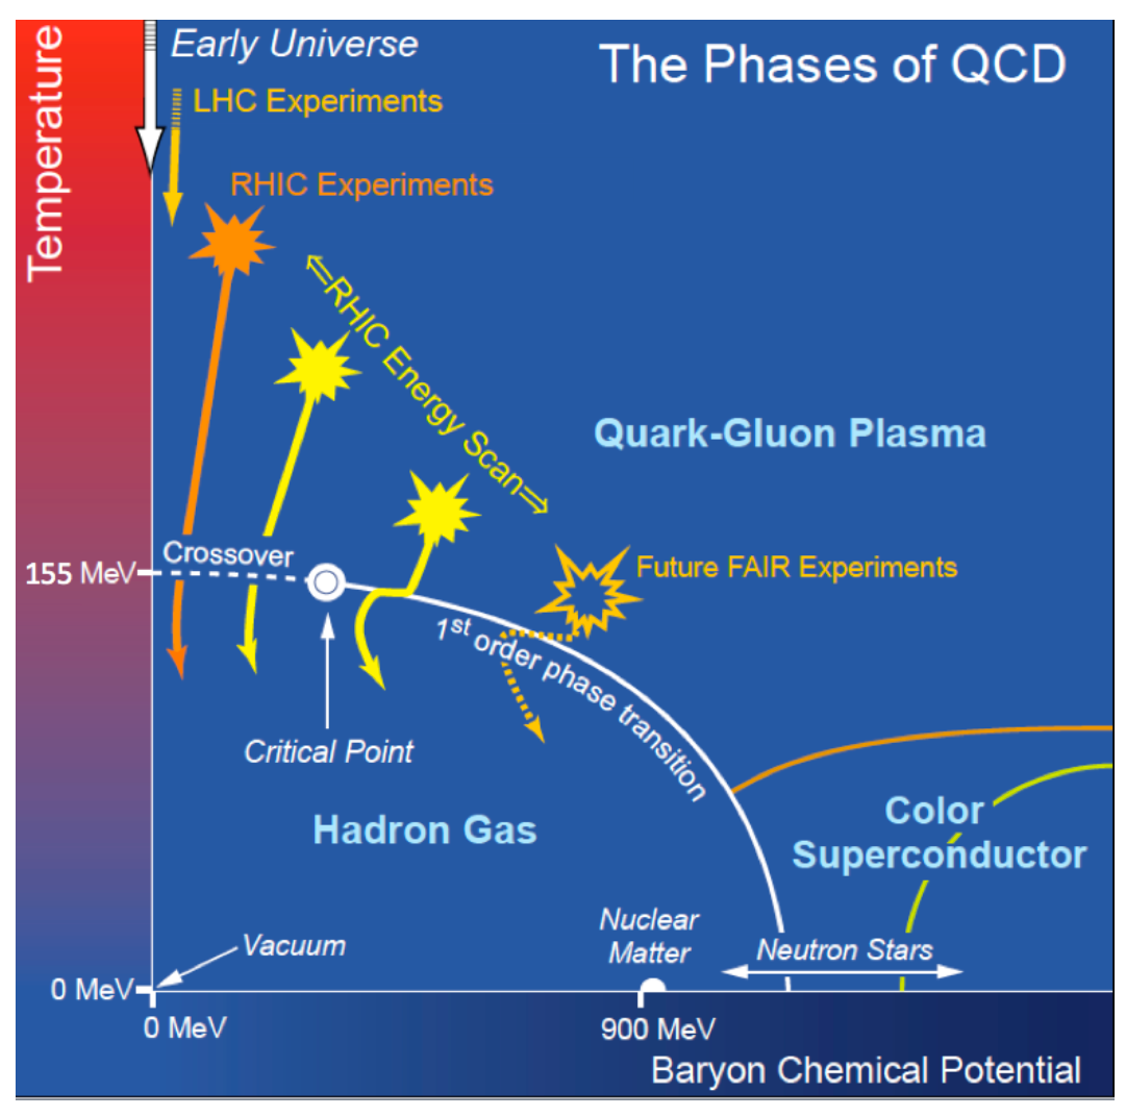
\includegraphics[width=0.7\textwidth,clip]{figures/Chapter1/PhaseDiagram.png}
    \end{center}
    \caption[QGP相图]{QGP相图}
    \label{fig:PhaseDiagram}
\end{figure}

QCD的相图给出来的是在温度T和重子化学势$\mu_b$平面上的热力学状态图,从图中可以看出,研究QCD物质相变时,有两种常见的路线。一种是在保持低温的情况下增加夸克物质的密度,沿着这条路线最后达到的物质状态即为中子星内部的物质状态。另一条路线是加热核物质,也可以达到从强子气到夸克胶子等粒子体的相变,这种方式一般通过相对论重离子对撞来实现。